\PassOptionsToPackage{lowtilde}{url}
\documentclass[aspectratio=43,english]{beamer} %If you want to create Polish presentation, replace 'english' with 'polish' and uncomment 3-th line, i.e., '\usepackage{polski}'
\usepackage[utf8]{inputenc}
\usepackage{polski} %Uncomment for Polish language
\usepackage{babel}
\usepackage{listings} %We want to put listings

\mode<beamer>{ 	%in 'beamer' mode
	\hypersetup{pdfpagemode=FullScreen}		%Enable Full screen mode
	\usetheme{JuanLesPins} 		%Show part title in right footer
	%\usetheme[dark]{AGH}                 		%Use dark background
	%\usetheme[dark,parttitle=leftfooter]{AGH}  	%Use dark background and show part title in left footer
}
\mode<handout>{	%in 'handout' mode
	\hypersetup{pdfpagemode=None}
	\usepackage{pgfpages}
  	\pgfpagesuselayout{4 on 1}[a4paper,border shrink=5mm,landscape]	%show 4 slides on 1 page
  	\usetheme{boxes}
  	\addheadbox{structure}{\quad\insertpart\hfill\insertsection\hfill\insertsubsection\qquad} 	%content of header
 	\addfootbox{structure}{\quad\insertauthor\hfill\insertframenumber\hfill\insertsubtitle\qquad} 	%content of footer
}

\AtBeginPart{ %At begin part: display its name
	\frame{\partpage}
}


%%%%%%%%%%% Configuration of the listings package %%%%%%%%%%%%%%%%%%%%%%%%%%
% Source: https://en.wikibooks.org/wiki/LaTeX/Source_Code_Listings#Using_the_listings_package
%%%%%%%%%%%%%%%%%%%%%%%%%%%%%%%%%%%%%%%%%%%%%%%%%%%%%%%%%%%%%%%%%%%%%%%%%%%%
\lstset{ %
  backgroundcolor=\color{white},   % choose the background color
  basicstyle=\footnotesize,        % the size of the fonts that are used for the code
  breakatwhitespace=false,         % sets if automatic breaks should only happen at whitespace
  breaklines=true,                 % sets automatic line breaking
  captionpos=b,                    % sets the caption-position to bottom
  commentstyle=\color{green},      % comment style
  deletekeywords={...},            % if you want to delete keywords from the given language
  escapeinside={\%*}{*)},          % if you want to add LaTeX within your code
  extendedchars=true,              % lets you use non-ASCII characters; for 8-bits encodings only, does not work with UTF-8
  frame=single,	                   % adds a frame around the code
  keepspaces=true,                 % keeps spaces in text, useful for keeping indentation of code (possibly needs columns=flexible)
  keywordstyle=\color{blue},       % keyword style
  morekeywords={*,...},            % if you want to add more keywords to the set
  numbers=left,                    % where to put the line-numbers; possible values are (none, left, right)
  numbersep=5pt,                   % how far the line-numbers are from the code
  numberstyle=\tiny\color{gray},   % the style that is used for the line-numbers
  rulecolor=\color{black},         % if not set, the frame-color may be changed on line-breaks within not-black text (e.g. comments (green here))
  showspaces=false,                % show spaces everywhere adding particular underscores; it overrides 'showstringspaces'
  showstringspaces=false,          % underline spaces within strings only
  showtabs=false,                  % show tabs within strings adding particular underscores
  stepnumber=2,                    % the step between two line-numbers. If it's 1, each line will be numbered
  stringstyle=\color{cyan},        % string literal style
  tabsize=2,	                   % sets default tabsize to 2 spaces
  title=\lstname,                  % show the filename of files included with \lstinputlisting; also try caption instead of title
                                   % needed if you want to use UTF-8 Polish chars
  literate={?}{{\k{a}}}1
           {?}{{\k{A}}}1
           {?}{{\k{e}}}1
           {?}{{\k{E}}}1
           {�}{{\'o}}1
           {�}{{\'O}}1
           {?}{{\'s}}1
           {?}{{\'S}}1
           {?}{{\l{}}}1
           {?}{{\L{}}}1
           {?}{{\.z}}1
           {?}{{\.Z}}1
           {?}{{\'z}}1
           {?}{{\'Z}}1
           {?}{{\'c}}1
           {?}{{\'C}}1
           {?}{{\'n}}1
           {?}{{\'N}}1
}
%%%%%%%%%%%%%%%%%
\setcounter{tocdepth}{1}

\newcommand\tab[1][0.5cm]{\hspace*{#1}}


\newcommand{\setcontributors}[1]{
	\let\oldmaketitle\maketitle
	\renewcommand{\maketitle}{
		\begin{frame}
			\oldmaketitle

			\noindent
				\begin{minipage}{0.4\textwidth}
						\footnotesize{\textbf{Contributors}}\\
						\scriptsize{#1}
						% \footnotesize{\textbf{Source code}}\\
						% 	\tab \scriptsize{\href{https://github.com/AGH-MOwNiT-2017/lectures}{\texttt{github.com/AGH-MOwNiT-2017/lectures}}}

				\end{minipage}
				\hfill%
				\begin{minipage}{0.45\textwidth}\raggedleft% adapt widths of minipages to your needs
					\includegraphics[width=25px, height=25px]{img/title/dice}
					\includegraphics[width=60px, height=35px]{img/title/ki}
					\includegraphics[width=30px, height=30px]{img/title/agh}

				\end{minipage}%


		\end{frame}
	}
}


\title{Metody Obliczeniowe w Nauce i Technice}
\author{Marian Bubak, Katarzyna Rycerz}
\date{}
\institute[AGH]{
	Department of Computer Science\\
	AGH University of Science and Technology\\
	Krakow, Poland\\
	\href{mailto:kzajac@agh.edu.pl}{\texttt{kzajac@agh.edu.pl}}\\
	% \href{http://www.icsr.agh.edu.pl/~mownit/}{\texttt{icsr.agh.edu.pl/$\sim$mownit}}
	\href{http://dice.cyfronet.pl/}{\texttt{dice.cyfronet.pl}}

}
\usepackage{amsmath}
\usepackage{mathtools}
\subtitle{4. Funkcje sklejane - spline functions}
\setcontributors{Mateusz Woś\\Michał Matusiak\\Kamil Doległo}


\begin{document}
  	\maketitle
	%%%%%%%%%%%%%%%%
	\begin{frame}{Outline}
		\tableofcontents
	\end{frame}
	%%%%%%%%%%%%%%%%
	\section{Wprowadzenie}
	\begin{frame}{Wprowadzenie}
	\begin{itemize}
	    \item 	wywodzą się z praktyki inżynierskiej
	    \item  do kreślenia elementów konstrukcyjnych w przemyśle  używano elastycznej listewki drewnianej (liniału) nazywanej giętką (ang.spline)
	    \item liniał prowadzono przez zadane punkty za pomocą  ciężarków
	    \item liniał uginał się wzdłuż krzywej „najgładszej”
	    \item  alternatywa: użycie krzywików
	   \end{itemize}
	   \begin{figure}
	       \centering
	       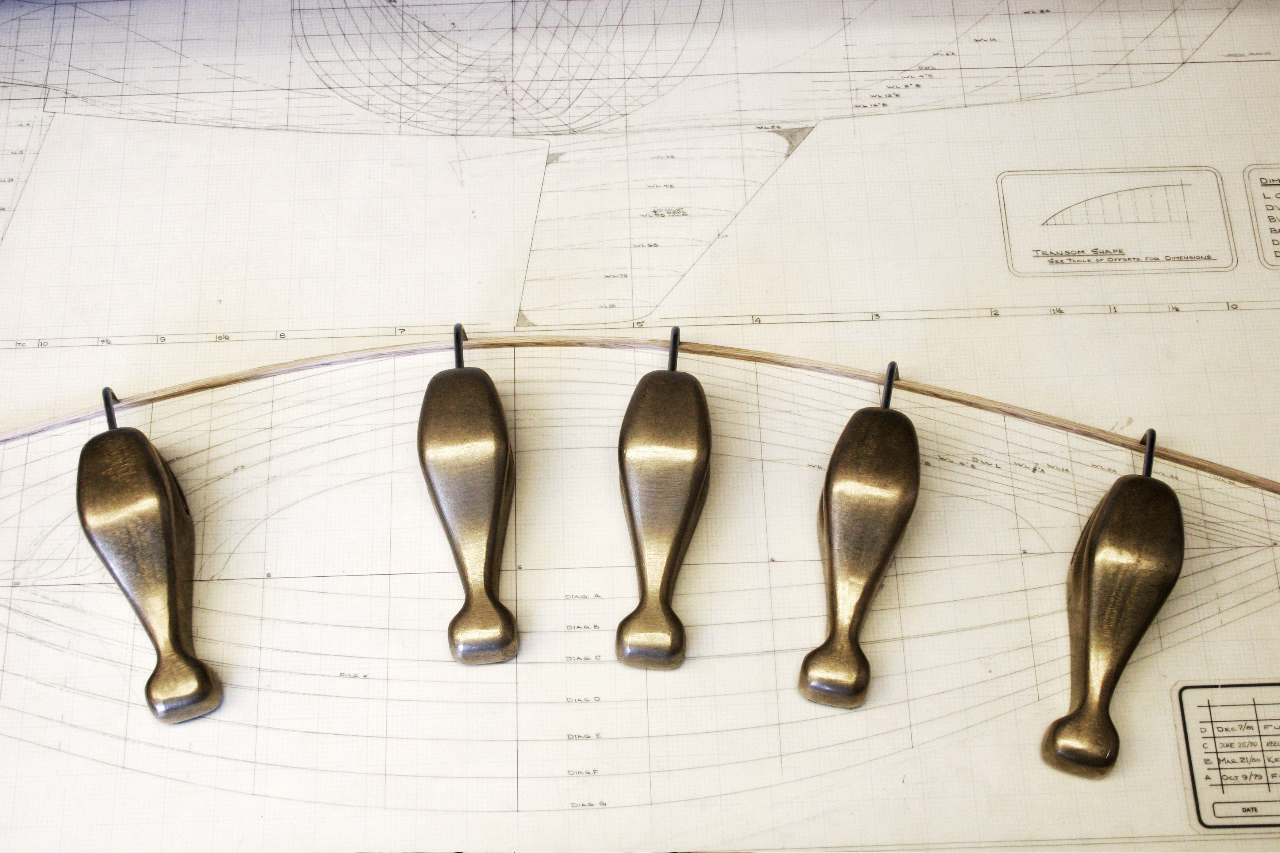
\includegraphics[width=4cm]{img/4/spline_figure.jpg}
	       \caption{źródło: http://www.alatown.com/spline/}
	       \label{fig:my_label}
	   \end{figure}
        
     %   $s(x)$ - funkcja $\newline$
     %   $s''(x)$ - krzywizna, dx - długość łuku $\newline$
     %   $s,\ s',\ s'' $ - ciągłe w $[x_{i},x_{n}] \newline$
     %   local curvature: $\frac{f''(x)}{(1+f'(x))^{\frac{5}{2}}}$
     %  \[
     %   	\min ! \int_{x_{i}}^{x_{n}}\underbrace{[s''(x)]^{2}dx}_{E_{p}}
      %      \Rightarrow w_{3}(x)
      %      \ \ \textrm{na} \ \ [x_{i},x_{i+1}]
      %  \]
      % \[
      %  	\textrm{"strain energy"} = \int_{a}^{b} 
      %      \frac{(f''(x))^{2}}{(1+f'(x))^{\frac{3}{2}}}dx
      %  \]
        
	\end{frame}
    %%%%%%%%%%%%%%%%%%%%%%%%%%%%%%%%%%%%%%%%%%%%%%%%%%
    \begin{frame}{Definicja funkcji sklejanej}
    	\begin{exampleblock}{}
    		Funkcję $s(x) = s(x, \Delta n)$ określoną na $[a,b]$ nazywamy funkcją sklejaną stopnia m $(m\geq1)$ jeżeli:
            \begin{itemize}
            \item $s(x)$ jest wielomianem stopnia $ \leq m$ na każdym $[x_{i},x_{i+1}]$
            \item $s(x) \in C^{m-1}[a,b] $
            \end{itemize}
            $\newline$
            $\Delta n$ - podział $[a,b]$ na (n-1) podprzedziałów przez węzły: 
            $a=x_{1}<x_{2}<...<x_{i}<...<x_{n}=b$
    	\end{exampleblock}
	
    \end{frame}
    \begin{frame}
    
		\begin{figure}[h]
			\includegraphics[width=.9\linewidth]{img/4/spline_img_4}
		\end{figure}
    \end{frame}
	%%%%%%%%%%%%%%%%%%%%%%%
	\section{Liniowa funkcja sklejana}
    %%%%%%%%%%%%%%%%%%%%%%%%%%%%%%%%%%%%5
    \begin{frame}{Liniowa funkcja sklejana}
        \begin{figure}[h]
			\includegraphics[width=.9\linewidth]{img/4/spline_img_1}
		\end{figure}
		
    \end{frame}
    
	\begin{frame}{Liniowa funkcja sklejana}
    	Interpolacja podziałowa, liniowa: Dla $x\in[x_{i},\ x_{i+1}]$:
       \[
		y(x)=y_{i}+\frac{y_{i+1}-y_{i}}{x_{i+1}-x_{i}}(x-x_{i})=\underbrace{\frac{x_{i+1}-x}{x_{i+1}-x_{i}}}_{\text{$\Psi_{i}$}}y_{i}+\underbrace{\frac{x-x_{i}}{x_{i+1}-x_{i}}}_{\text{$\Psi_{i+1}$}}y_{i+1}(*)
		\]
        %%%%%%%%%%%%%%%%%%%%%%%%
        $\newline$
        Dla $x\in[x_{i-1},\ x_{i}]:$
       \[
		y(x)=\underbrace{\frac{x_{i}-x}{x_{i}-x_{i-1}}}_{\text{$\Psi_{i-1}$}}y_{i-1}+\underbrace{\frac{x-x_{i-1}}{x_{i}-x_{i-1}}}_{\text{$\Psi_{i}$}}y_{i}
		\]
        $\newline$
        \textbf{Funkcja kształtu} (shape function)
        \[
        	\Psi_{i}(x) = 
            \begin{cases}
            	\frac{x-x_{i-1}}{x_{i}-x_{i-1}} &x \in [x_{i-1},x_{i}] 
            	\\
                \frac{x_{i+1}-x}{x_{i+1}-x_{i}} &x \in [x_{i},x_{i+1}] 
             	\\
            	0 &x  \notin [x_{i-1},x_{i+1}]   
            \end{cases}
        \]
        	\end{frame}
        \begin{frame}
        	\begin{figure}[h]
			\includegraphics[width=.6\linewidth]{img/4/spline_img_2}
		\end{figure}
             %%%%%%%%%%%%%%%%%%%%%%%%
		\begin{alertblock}{\textbf{Ważne}}
			$\Psi_{i}(x_{j})=
            \begin{cases} 0 \ dla \ j\neq i \\1 \ dla \ j=i \end{cases}$
		\end{alertblock}
        \end{frame}
        

    
    
    
   %%%%%%%%%%%%%%%%%%%%%%%%%%%%%%%5
   \begin{frame}{Funkcje B-sklejane 1 stopnia}
   		\begin{exampleblock}{}
   			Interpolującą funkcję sklejaną stopnia 1-go można zapisać:
            \[
            	s(x)=\sum_{i=0}^{n}y_{i}\Psi_{i}(x)
            \]
            gdzie $\Psi_{i}(x), i=0,...,n$ - baza przestrzeni liniowej funkcji sklejanych
            1-go stopnia
   		\end{exampleblock}
        \begin{figure}[h]
			\includegraphics[width=.65\linewidth]{img/4/spline_img_3}
		\end{figure}
   \end{frame}
    
    
    
    
    
    
    
    
    
    
    
    
    
    
    
    
    
    
	%%%%%%%%%%%%%%%%%%%%%%%
	\section{Interpolacja sześcienna (cubic spine)}
	\begin{frame}{Interpolacja sześcienna (cubic spine)}
	 W praktyce najczęściej używane.
		\begin{block}{}
			\begin{itemize}
				\item $s_{i}$ on $[x_{i},x_{i+1}] \rightarrow$ cubic polynomial:
                $\newline \ \ \ s_{i}(x)=a_{i}+b_{i}(x-x_{i})+c_{i}(x-x_{i})^{2}+
                d_{i}(x-x_{i})^{3}$
                \item $s_{i}(x_{i+1})=f(x_{i+1})$
                \item $s_{i}(x_{i+1})=s_{i+1}(x_{i+1})$
                \item $s^{'}_{i}(x_{i+1})=s^{'}_{i+1}(x_{i+1})$
                \item $s^{''}_{i}(x_{i+1})=s^{''}_{i+1}(x_{i+1})$
			\end{itemize}
		\end{block}
		
		
		Wypisując takie warunki dla każdego z "wewnętrznych"  punktów intepolacji i dodając warunki brzegowe można stworzyć układ równań i go rozwiązywać\\
		Istnieje jednak sprytniejsze podejście !
        
	\end{frame}
	%%%%%%%%%%%%%%%%%%%%%%%
\section{Konstrukcja interpolujących sześciennych funkcji sklejanych}
	
	\begin{frame}{Konstrukcja interpolujących sześciennych funkcji sklejanych}

     Ponieważ $s_i(x)$ - sześcienna, \\
     	  to $s''_i(x)$ -liniowa na przedziale $[x_{i},x_{i+1}] $\\
	 wprowadzam $h_{i}=x_{i+1}-x_{i}$, wtedy (z (*)):\\
	 \vspace{3mm}
	   \begin{center}
	  $s_i^{''}(x)=s_i^{''}(x_i)\frac{x_{i+1}-x}{h_i}+s_i^{''}(x_{i+1})\frac{x-x_i}{h_i}$(**)\\
	  	  \end{center}
	  całkując dwukrotnie otrzymuję:\\
	  \begin{center}
	       $s_i(x)=\frac{s_i^{''}(x_i)}{6h_i}(x_{i+1}-x)^3+\frac{s_i^{''}(x_{i+1})}{6h_i}(x-x_i)^3+C(x-x_i)+D(x_{i+1}-x)$, 
	  \end{center}
	   gdzie C, D - stałe całkowania.\\
	  korzystając z  warunków interpolacji :\\
	  $s_i(x_i)=y_i$ oraz $s_i(x_{i+1})=y_{i+1}$ mogę wyliczyć C i D 
	  	\end{frame}
	  \begin{frame}
	   Po wyliczeniu C i D z  warunków interpolacji mamy:\\
	  $s_i(x)=\frac{s_i^{''}(x_i)}{6h_i}(x_{i+1}-x)^3+\frac{s_i^{''}(x_{i+1})}{6h_i}(x-x_i)^3+
	  (\frac{y_{i+1}}{h_i}-\frac{z_{i+1}h_i}{6})(x-x_i)+(\frac{y_i}{h_i}-\frac{z_ih_i}{6})(x_{i+1}-x)$  \\
		 \vspace{3mm}
	 W powyższym wzorze nie znamy $s_i^{''}(x)$ . Aby je wyliczyć korzystamy z warunku ciągłości pierwszej pochodnej. Różniczkujemy więć $s_i(x)$\\
	 	 \vspace{3mm}
	 $s_i^{'}(x_i)=-\frac{h_i}{3}s_i^{''}(x_i)-\frac{h_i}{6}s_i^{''}(x_{i+1})-\frac{y_i}{h_i}+\frac{y_{i+1}}{h_i}$\\
	 	 \vspace{3mm}
	    Dla przejrzystości wprowadzamy symbole: $\sigma_{i}=\frac{1}{6}s''(x_{i})$ oraz $\Delta_{i}=\frac{y_{i+1}-y_{i}}{h_{i}} $ (uwaga: $\Delta$ oznacza co innego niż na poprzednim wykładzie), wtedy: \\
	     \vspace{3mm}
	    $s_i^{'}(x_i)=-2\sigma_{i}h_i-\sigma_{i+1}h_i+\Delta_{i}$\\
        $ s_{i}'(x_{i})  &=\ \Delta_{i}-h_{i}(\sigma_{i+1}+2\sigma_{i})$\\
        Natomiast    od drugiej strony:\\   	
        $s_{i-1}'(x_{i}) &=\ \Delta_{i-1}+h_{i-1}(2\sigma_{i}+\sigma_{i-1})$\\
        \end{frame}
        
        
        
        \begin{frame}
        \begin{block}{}
        	\centering Warunek ciągłości: $s_{i-1}'(x_{i}) = s_{i}'(x_{i})$
        \end{block}
        \[
        	\framebox{$\Delta_{i-1}+h_{i-1}(2\sigma_{i}+\sigma_{i-1})=
            \Delta_{i}-h_{i}(\sigma_{i+1}+2\sigma_{i})$}
        \]
        otrzymujemy układ (n-2) równań liniowych  (dla punktów pośrednich):
        \[
        	h_{i-1}\sigma_{i-1}+2(h_{i-1}+h_{i})\sigma_{i}+h_{i}\sigma_{i+1}=
            \Delta_{i}-\Delta_{i-1}, \ \ i=2, 3, . . . , n-1
        \]
        ale ponieważ mamy n niewiadomych $\sigma_{i}$ konieczne jest
        określanie dwóch dodatkowych warunków.
    \end{frame}
    %%%%%%%%%%%%%%%%%%%%%%%
    \begin{frame}
		$\newline$
    	Istnieje wiele sposobów określania dodatkowych warunków.
       \begin{enumerate}
       \item  \[
		\begin{rcases*}
			C_{1}(x) - \textrm{f. sześcienna przez pierwsze 4 punkty}\\
			C_{n}(x) - \textrm{f. sześcienna przez ostatnie 4 punkty}
		\end{rcases*} \rightarrow
		\]	
       \end{enumerate}	
       \[
       		\framebox{$s'''(x_{1})=C^{'''}_{1}\ \ \ s'''(x_{n})=C^{'''}_{n}$}
       \]
        Stałe $C^{'''}_{1}$ i $C^{'''}_{n}$ mogą być określone bez znajomości 
        $C_{1}(x)$ i $C_{n}(x)$:
        \[
        	\Delta_{i}\ =\ \frac{y_{i+1}-y_{i}}
            {x_{i+1}-x_{i}}\ ;\ \textrm{przybliża 1-szą pochodną}
        \]
        \[
        	\Delta_{i}^{(2)}=\frac{\Delta_{i+1}-\Delta_{i}}
            {x_{i+2}-x_{i}}\ ;\ 2\Delta_{i}^{(2)}\approx f^{''}
        \]
        \[
        	\Delta_{i}^{(3)}\ =\ \frac{\Delta_{i+1}^{(2)}-\Delta_{i}^{(2)}}
            {x_{i+3}-x_{i}}\ ;\ 6\Delta_{i}^{(3)}\approx f^{'''}
        \]
    \end{frame}
    %%%%%%%%%%%%%%%%%%%%%%
    \begin{frame}
    	i ogólnie dla ilorazów róznicowych:
        \begin{flushright}
        	$\Delta_{0}^{(0)}=f[x_{0}]\equiv f(x_{0}) \linebreak \linebreak$
            $\Delta_{0}^{(1)}=f[x_{0},\ x_{1}]\equiv\frac{f[x_{1}]-f[x_{0}]}{x_{1}-
            x_{0}}=\frac{f(x_{1})-f(x_{0})}{x_{1}-x_{0}} 
            \linebreak \linebreak$
            $\Delta_{0}^{(3)}=f[x_{0},\ x_{1},\ x_{2}]\equiv\frac{f[x_{1},x_{2}]-f[x_{0},x_{1}]}
            {x_{2}-x_{0}} \linebreak $
            $\ldots \ldots \linebreak$
            $\Delta_{0}^{(n)}=f[x_{0},\ x_{1},\ .\ .\ .\ ,\ x_{k}]\equiv\frac{f[x_{1},\ldots,x_{k}]-f[x_{0},\ldots,x_{k-1}]}{x_{k}-x_{0}}$
        \end{flushright}
        mamy związek między ilorazami różnicowymi a pochodnymi:
        \begin{exampleblock}{}
        	$
            	\centering f[x_{0}, ... \ , x_{n}]=\frac{f^{(n)}(\eta)}
                {n!}, \ \ \ \eta \in [x_{0},... \ , x_{n}]
                \ \ \ (\eta \textrm{- pewien punkt})
            $
        \end{exampleblock}
        \begin{block}{Przypomnienie}
         To wynika z 	uogólnionego  twierdzenie o wartości średniej (poprzedni wykład) 
        \end{block}
        
    \end{frame}
    %%%%%%%%%%%%%%
    \begin{frame}
    	Różniczkując wzór na $s^{''}(x)$ w przedziale $[x_{i},x_{i+1}] $ (**) otrzymujemy:
        $s_i^{'''}(x)=\frac{-s_i^{''}(x_i)}{h_i}+\frac{s_i^{''}(x_{i+1})}{h_i}=\frac{-6\sigma_{i}}{h_i}+\frac{6\sigma_{i+1}}{h_i}$\\
        Wtedy:
        \begin{align*}
        	s'''(x_{1})&=c_{1}'''(x_{1}) \Rightarrow
            \frac{6}{h_{1}}(\sigma_{2}-\sigma_{1})=6\Delta_{1}^{(3)}
            &|\cdot h_{1}^{2}
            \\
            s'''(x_{n})&=c_{n}'''(x_{1}) \Rightarrow
            \frac{6}{h_{n-1}}(\sigma_{n}-\sigma_{n-1})=6\Delta_{n-3}^{(3)}
            &|\cdot h_{n-1}^{2}
        \end{align*}
        po przekształceniu: (cel = symetria)
        $\newline \newline
        \begin{cases}
        	-h_{1}\sigma_{1}+h_{1}\sigma_{2}=h_{1}^{2}\Delta_{1}^{(3)}
            \\
		h_{n-1}\sigma_{n-1}-h_{n-1}\sigma_{n}=-h_{n-1}^{2}\Delta_{n-3}^{(3)}
        \end{cases}
        $
    \end{frame}
    %%%%%%%%%%%%%%%%%%
    \begin{frame}
    	mamy:
        \[
        \begin{bmatrix}
    -h_{1} & h_{1} & 0 & 0  & 0 \\
    h_{1} & 2(h_{1}+h_{2}) & h_{2} & 0  & 0 \\
    0 & h_{2} & 2(h_{2}+h_{3}) & h_{3} & 0 \\
    \vdots & \vdots & \vdots & \vdots & \vdots \\
    0 & 0 & h_{n-2} & 2(h_{n-2}+h_{n-1}) & h_{n-1} \\
    0 & 0 & 0 & h_{n-1}  & -h_{n-1}
		\end{bmatrix}
        \begin{bmatrix}
        	\sigma_{1} \\
            \sigma_{2} \\
            \sigma_{3} \\
            \vdots \\
            \sigma_{n-1} \\
            \sigma_{n}
        \end{bmatrix}
       	=
        \]
        \[	=
        	\begin{bmatrix}
        		h_{1}^{2}\Delta^{(3)}_{1} \\
                \Delta_{2} - \Delta_{1} \\
                \Delta_{3} - \Delta_{2} \\
                \vdots \\ 
                \Delta_{n-1} - \Delta_{n-2} \\
                -h_{n-1}^{2}\Delta^{(3)}_{n-3}
        	\end{bmatrix}
        \]
    \end{frame}
    %%%%%%%%%%%%%%%%%%
    \begin{frame}{Inne ważne możliwości określania warunków}
    	\begin{itemize}
    		\item natural cubic spline: $s''(x_{1})=s''(x_{n})=0$ (free boundary)
            \item clamped boundary: $s'(x_{1})=f'_{1}, \ \ s'(x_{n})=f'_{n}$ (pierwsze pochodne na krańcach znane bądź przybliżone ilorazami różnicowymi)
            \item $s''(x_{1})=y''_{1}; \ \ s^{n}(x_{n})=y''_{n}$ (drugie pochodne na krańcach znane bądź przybliżone ilorazami różnicowymi, szczególny przypadek to natural cubic splines)
            \item not-a-knot condition $s'''_1(x_2)=s'''_2(x_2)$ oraz $s'''_{n-1}(x_{n-1})=s'''_{n}(x_{n-1})$  czyli $s'''(x)$ ciągła w $x_{2}$ oraz $x_{n-1}$
            \item interpolowanie spline'ami funkcji periodycznych
            $s(x_1)=s(x_n)$,
            $s'(x_1)=s'(x_n)$ oraz
            $s^{''}(x_1)=s^{''}(x_n)$
    	\end{itemize}
    \end{frame}
    %%%%%%%%%%%%%%%%%%%%
    \begin{frame}
    
        	Dla obliczeń - zwłaszcza wielokrotnego określania wartości s(x) 
            korzystna jest postać:
            \[
            	s(x)=y_{i}+b_{i}\cdot(x-x_{i})+c_{i}
                \cdot(x-x_{i})^{2}+d_{i}\cdot(x-x_{i})^{3}
                \ \ dla \ x\in[x_{i},\ x_{i+1}]
            \]
            $b_{i}, c_{i}, d_{i}$ - określone dla każdego przedziału:
            $b_{i}=\frac{y_{i+1}-y_{i}}{h_{i}}-h_{i}\cdot (\sigma_{i+1}
            +2\sigma_{i})\newline$
            $c_{i}=3\cdot \sigma_{i}\newline$
            $d_{i}=\frac{\sigma_{i+1}-\sigma_{i}}{h_{i}}\newline$

        
    \end{frame}
    %%%%%%%%%%%%%%%%%%%%
    \begin{frame}{Błąd interpolacji funkcji sklejanych}
    	Przykładowo dla {\it clamped boundary condition} udowodniono :
        \begin{itemize}
        \item $a=x_{1}, x_{2}, . . . , x_{n}=b$
        \item $f\in C^{4}[a,\ b] , \ \ \ \ \max_{x\in[a,b]}|f^{(4)}
        (x)|\leq M$
        \item $s'(x_{1})=f'(x_{1}), \ \ \ s'(x_{n})=f'(x_{n})$
        \end{itemize}
        to:
        \[
        	\max_{x\in[a,b]}|f(x)-s(x)|\leq \frac{5}{384} \cdot
            M \cdot \max_{1 \leq i \leq n-1}(x_{i+1}-x_{i})^{4}
        \]
        
        Wniosek:  jeśli dodamy 10 razy więcej punktów intepolacji, długość przedziału 
        $x_{i+1}-x_{i}$ zmniejszy się 10-krotnie, a ograniczenie górne błedu zmniejszy się $10^4$ razy !\\
        \small{
        Dowód A. Hall, W. Weston Meyer "Optimal error bounds for cubic spline interpolation",  \url{https://www.sciencedirect.com/science/article/pii/002190457690040X})}
    \end{frame}
    
    
    
    
    
    
    
    
    
    
    
    
    
    
    
    
    
    
    
    
    
    

    
    
    
    
    
    
    
    
    
    
    
    
    
    
    
    
    
    
    
	%%%%%%%%%%%%%%%%%%%%%%%
	\section{Zalety funkcji sklejanych}
\begin{frame}{Zalety}
	\begin{itemize}
	\item dokładniejsza, bezpieczniejsza interpolacja - patrz rysunek!
    \begin{figure}[h]
			\includegraphics[width=.75\linewidth]{img/4/spline_img_5}
		\end{figure}
	\end{itemize}
\end{frame}
%%%%%%%%%%%%%%%%
\begin{frame}{Zalety c.d.}
	\begin{itemize}
		\item wartości $s_{3}(x)$ łatwe do wyznaczania
    	\item w praktyce - $s_{3}$ wystarczające
    	\item przydatne dla węzłów równoodległych
    	\item można używać dla określenia $\Rightarrow \frac{d^{(n)}}	
        	{dx^{n}}f(x)$
    		i $\int f(x)dx$ 
	\end{itemize}
	
\end{frame}
%%%%%%%%%%%%%%%%
%\begin{frame}{Zastosowania}
%	\begin{itemize}
%		\item do wygładzania powierzchni:
 %       	\begin{itemize}
%        		\item siatka prostokątna $(x_{i},y_{i})$, $i=1,2,...,m$; 
 %               	$j=0,1,...,n$
 %               \item funkcje sklejane na siatce, np.: 
 %               \[
 %               	\framebox{$s(x,y)=\sum_{i=0}^{m}\sum_{j=0}^{n}f(x_{i},
 %                   \ y_{i})\psi_{i}(x)\psi_{j}(y)$}
 %               \]
 %               %% dead link
 %       	\end{itemize}
%	\end{itemize}
%\end{frame}
%%%%changed encoding of file, utf-8 -> utf-8(without BOM)








	%%%%%%%%%%%%%%%%%%%%%%%
	\section{B-splines - basic splines}
\begin{frame}{Funkcje B-sklejane}
    \begin{itemize}
        \item stosowane w grafice komputerowej do modelowania figur o skomplikowanych kształtach
        \item bazują na fakcie, że funkcje sklejane można wyrazić za pomocą kombinacji liniowej funkcji bazowych 
        \item takie funkcje bazowe nazywamy funkcjami B-sklejanymi (B-splines)
        \item dla danego zestawu  węzłów interpolacji - funkcje bazowe łatwo wyliczyć rekurencyjnie 
        \item algorytmy o dobrych własnościach numerycznych
    \end{itemize}
\end{frame}
\begin{frame}{Funkcje B-sklejane}
	$B_{j,k}(x)$ - B-spline rzędu k:
    \begin{itemize}
    \item  $B_{j,0}=
        \begin{cases}
            	1  &,\ x_{j} \leq x \leq x_{j+1}
            	\\
                0 &,\ \textrm{poza przedziałem}
        \end{cases}
        $
        \item wyższe rzędy $(k>0)$ - rekurencyjnie:
        \[
        	B_{j,k}(x)=\frac{x-x_{j}}{x_{j+k}-x_{j}}B_{j,k-1}(x)+\frac{x_{j+k+1}-x}
            {x_{j+k+1}-x_{j+1}}B_{j+1,k-1}(x)
        \]
        \item np. $B_{j,1}=\Psi_j$ (patrz interpolacja liniową funkcją sklejaną)
    \end{itemize}
    \begin{exampleblock}{Reprezentacja funkcji sklejanej stopnia k}
		\centering $S(x)=\sum_{j}p_{j}B_{j,k}(x)$
	\end{exampleblock}
	 gdzie $p_j$ - wspólczynniki (w grafice komputerowej są to tzw. zadane punkty kontrolne) 
\end{frame}
%%%%%%%%%%%%%%%%%%%%%%%%%%%%%%%%%%%%%%%%%%%%%%
\begin{frame}{Funkcje B-sklejane - własności}
     \begin{itemize}
        \item $B_{j,k}(x)>0, x\in[x_{j} \ x_{j+k+1}]$ 
        \item $B_{j,k}(x)=0, x\notin[x_{j} \ x_{j+k+1}]$ 
       
        \item w przedziale $[x_{j},\ x_{j+1}]$ istotne jest tylko $k+1$ funkcji : $B_{j-k,k}(x)\ldots  B_{j,k}(x)\neq 0$
		\item normalizacja: $\sum_{j}B_{j,k}(x)=\sum_{j=l-k}^{l}B_{j,k}(x)=1$ 
        \newline dla $x_{l}\leq x\leq x_{l+1}$
    \end{itemize}
\end{frame}
%%%%%%%%%%%%%%%%%%%%%%%%
\begin{frame}{Funkcje B-sklejane stopnia 3}
	\begin{figure}[h]
			\includegraphics[width=.57\linewidth]{img/4/spline_img_6}
	\end{figure}
    \[\underbrace{B_{j,3}(x)}_{b_j(x)}=
    	\begin{cases}
    		\frac{1}{6}z^{3} &,z=\frac{x-x_{j}}{d} \ \ x \in [x_{j},x_{j+1}] \\
            \frac{1}{6}[1+3(1+z(1-z))z] &,z=\frac{x-x_{j+1}}{d} \ x 
            \in [x_{j+1},x_{j+2}]\\
            \frac{1}{6}[1+3(1+z(1-z))(1-z)] &,z=\frac{x-x_{j+2}}{d} \ x 
            \in [x_{j+2},x_{j+3}] \\
            \frac{1}{6}(1-z)^{3} &,z=\frac{x-x_{j+3}}{d} \ x 
            \in [x_{j+3},x_{j+4}] \\
            0 \ &, x \notin [x_{j},x_{j+4}]
    	\end{cases}
    \]
\end{frame}






	%%%%%%%%%%%%%%%%%%%%%%%
	%\input{4_spline/4_7_Literatura}
	%%%%%%%%%%%%%%%%%%%%%%%
\end{document}
